\documentclass[10pt]{article}

\usepackage{amsmath,amscd}
\usepackage{amssymb,array}
\usepackage{amsfonts,latexsym}
\usepackage[mathscr]{euscript}
\usepackage{graphicx,subfig,wrapfig}
\usepackage{times}
\usepackage{psfrag,epsfig}
\usepackage{verbatim}
\usepackage{tabularx}

\newcommand{\matlab}[1]{\texttt{#1}}
\newcommand{\setname}[1]{\textsl{#1}}
\newcommand{\Ce}{\mathbb{C}}
\newcommand{\Ree}{\mathbb{R}}
\newcommand{\p}{\begin{pmatrix}}
\newcommand{\pp}{\end{pmatrix}}
\newcommand{\bm}{\begin{bmatrix}}
\newcommand{\bb}{\end{bmatrix}}
\newcommand{\eul}[1]{e^{#1}}

\begin{document}

\title{ \vspace{-30mm}Systems Bioengineering 3\\Homework 13}
\author{Greg Kiar}

\maketitle
\begin{enumerate}
\item
\begin{enumerate}
\item Solving for $P_n$ yeilds
\begin{align*}
\beta P_n &= \alpha(n+1) P_{n+1} \\
P_1 &= \frac{\beta}{\alpha}P_{0}\\
P_2 &= \frac{\beta}{\alpha}P_{1} =  \frac{1}{2}\begin{pmatrix}\frac{\alpha}{\beta} \end{pmatrix}^2P_0 \\
\vdots \\
P_n &= \frac{1}{n!} \begin{pmatrix} \frac{\beta}{\alpha}\end{pmatrix}^n P_0 \\
1 &= \sum_{i=1}^{\infty}  \frac{1}{n!} \begin{pmatrix} \frac{\beta}{\alpha}\end{pmatrix}^n P_0\\
P_0 &= \frac{1}{\sum_{i=1}^{\infty}  \frac{1}{n!} \begin{pmatrix} \frac{\beta}{\alpha}\end{pmatrix}^n} \\
P_0 &= e^{-\frac{\beta}{\alpha}}\\
\therefore P_n &= \frac{1}{n!} \begin{pmatrix} \frac{\beta}{\alpha}\end{pmatrix}^n e^{-\frac{\beta}{\alpha}}
\end{align*}
\item Expressing $\tilde{P}(\phi)$ as a closed form solutions is done as follows
\begin{align*}
\tilde{P}(\phi) &= \sum_{n=0}^{\infty}e^{-\phi n}P_n \\
&= \sum_{n=0}^{\infty}e^{-\phi n} \frac{1}{n!} \begin{pmatrix} \frac{\beta}{\alpha}\end{pmatrix}^n e^{-\frac{\beta}{\alpha}}\\
&= e^{-\frac{\beta}{\alpha}} \sum_{n=0}^{\infty} \frac{\begin{pmatrix}\frac{\beta e^{-\phi}}{\alpha}\end{pmatrix}^{n}}{n!}  \\
\tilde{P}(\phi) &= e^{\frac{\beta}{\alpha} (e^{-\phi} - 1)} \\
\end{align*}
From this expression, and the definition of the mean and variance (stated below), we compute the mean and variance of this system
\begin{align*}
\langle n \rangle &= \frac{-d}{d \phi} \ln \tilde{P}(\phi) \vert_{\phi = 0}\\
&= \frac{-d}{d \phi} \begin{pmatrix} \frac{\beta}{\alpha} (e^{-\phi} - 1)\end{pmatrix}\\ \langle n \rangle &= \frac{\beta}{\alpha}\\
var(n) &= \langle n^2 \rangle - \langle n\rangle^2 = \frac{d^2}{d \phi^2} \ln \tilde{P}(\phi) \vert_{\phi = 0}\\
&= \frac{d^2}{d \phi^2}  \begin{pmatrix} \frac{\beta}{\alpha} (e^{-\phi} - 1)\end{pmatrix}\\
\langle n^2 \rangle - \langle n\rangle^2 &= \frac{\beta}{\alpha}
\end{align*}
\item From state $n$, in one transition only states $n+1$ and $n-1$ can be reached; however, over an infinite amount of time any state can be reached by this system.The probability distribution of this system is given by $P(t)$, which can be solved to find the mean time for the first transition, $\tau$.
\begin{align*}
P(\tau) &= (\beta + \alpha n)e^{-(\beta+\alpha n) t} \\
\tau &= \int_0^{\infty}t P(t) dt \\
\tau &= \frac{1}{\beta + \alpha n} \\
\end{align*}
\item Mapping this stochastic dynamic onto a continuous function yeilds the following
\begin{align*}
\dot{X}(t) &= \beta - \alpha X(t) \\
sX(s) - X(0) &= \frac{\beta}{s} - \alpha X(s) \\
X(s) &= \frac{\beta}{s(s+\alpha)} + \frac{\frac{\beta}{\alpha}}{s+ \alpha} \\
X(t) &= \frac{\beta}{\alpha}\\
\end{align*}
Since $X(t) = \frac{\beta}{\alpha}$ for all $t$, the mean of this system $\langle t \rangle = \frac{\beta}{\alpha}$, and the variance $\langle t^2 \rangle - \langle t \rangle^2 = 0$.
\end{enumerate}
\clearpage
\item
\begin{enumerate}
\item As can be seen from part 2b) above, the variance of $n$ takes the form of $\frac{\beta}{\alpha}$, so the variance here is $S(0) = 10$. Since the relaxation of $X(t)$ is defined, we can compute $S(t)$.
\begin{align*}
X(t) &= \frac{\beta}{\alpha}(1-e^{-\alpha t}) + X(0)e^{-\alpha t} \\
S(t) &= \frac{X(t) - \mu}{X(0) - \mu} S(0) \\
&= S(0)e^{-\alpha t} \\
&= \frac{\beta}{\alpha}e^{-\alpha t} \\
&= 10 e^{-\alpha t}
\end{align*}
\item The value of $\langle n \rangle$ is approximately $10$. You can see from the figure below that the two plots are identical to one another - the two being the analytical and experimental solutions to this equation.
\begin{center} 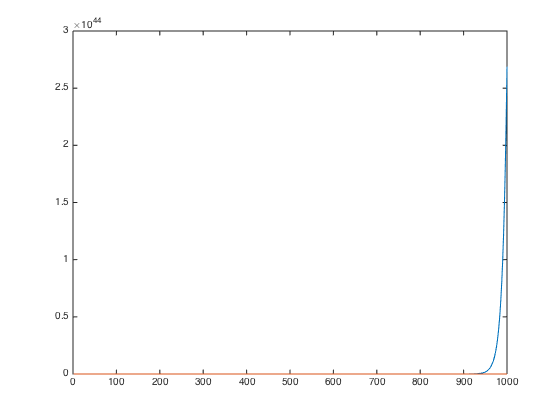
\includegraphics[scale=0.4]{sbe3hw13q2b.png} \end{center}
\item
\end{enumerate}
\item
\begin{enumerate}
\item The nullclines for the equations given above were found to be: \begin{align*} Y(t) &= \begin{pmatrix} \frac{2}{X(t)} - 1 \end{pmatrix}^{\frac{1}{n}} ;& \text{nullcline for } \dot{X}(t) = 0 \\ Y(t) &= \frac{2}{1+ X(t)^m} ;& \text{nullcline for } \dot{Y}(t) = 0 \end{align*}
The nullclines of plotted for values of $n = (1, 2, 4)$ and $m = (2)$ are as follows.
\begin{center} 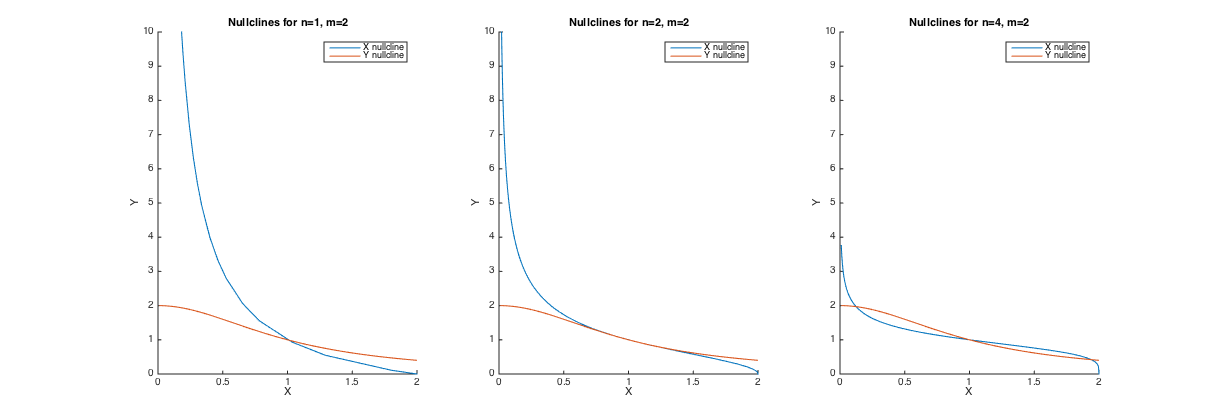
\includegraphics[scale=0.25]{sbe3hw13q3a.png} \end{center}
\item For the case when $n=4$ and $m=2$, we notice that the nullclines cross at three locations. If we compute the roots of the system $Z = Y_{null} - X_{null}$ we can find the locations where the two nullclines intersect. Performing this analysis the roots were found to be: $(0.1247, 1.9694)$, $(1,1)$, $(1.9397, 0.4200)$, where the center/symmetric fixed point occurs at $(1,1)$. Shown below is a plot of this system with the fixed points found above marked on the plot. \begin{center} 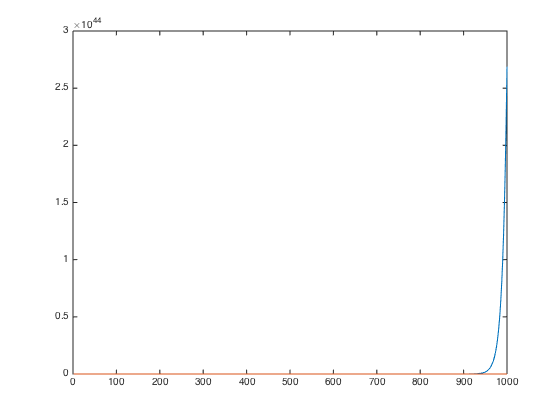
\includegraphics[scale=0.3]{sbe3hw13q2b.png} \end{center}
\item The Jacobian of this system can be computed as follows. \begin{align*}
J &= \begin{bmatrix} \frac{\partial \dot{X}}{\partial X} & \frac{\partial \dot{X} }{\partial Y} \\ \\ \frac{\partial \dot{Y}}{\partial X} & \frac{\partial \dot{Y}}{\partial Y} \end{bmatrix}\\
 &= \begin{bmatrix} -1 & \frac{-2nY^{n-1}}{(1+Y^n)^2} \\ \\  \frac{-2nX^{m-1}}{(1+X^m)^2} & -1 \end{bmatrix}\\
\end{align*}
We can simplify the above, and evaluate it at the fixed point $(1,1)$ \begin{align*}
J &= \begin{bmatrix} -1 & \frac{nX^2Y^{n-1}}{2} \\ \\  \frac{mY^2X^{m-1}}{2} & -1 \end{bmatrix}_{(1,1)}\\
J &= \begin{bmatrix} -1 & \frac{n}{2} \\ \\  \frac{m}{2} & -1 \end{bmatrix}
\end{align*}
The eigen values can be computed by solving $0 = \lvert J - \lambda I \rvert$
\begin{align*}
0 &= \begin{vmatrix} \begin{bmatrix} -1 & \frac{n}{2} \\ \\  \frac{m}{2} & -1 \end{bmatrix} - \begin{bmatrix} \lambda & 0 \\ \\  0 & \lambda \end{bmatrix} \end{vmatrix} \\
0 &= \begin{vmatrix} -1 - \lambda & \frac{n}{2} \\ \\  \frac{m}{2} & -1 -\lambda \end{vmatrix} \\
0 &= (-1 - \lambda)^2 - \frac{m n}{4} \\
\lambda &= -1 \pm \sqrt{\frac{mn}{4}}
\end{align*}
In order for the fixed point to be unstable, the following condition must apply
\begin{align*}
0 &< \lambda \\
0 &< -1 + \sqrt{\frac{mn}{4}} \\
1 &< \sqrt{\frac{mn}{4}} \\
4 &< mn
\end{align*}
The condition on the Hill coefficients that permits patterning is a large number of components combine between the two systems. If the product of the system compontents is larger than $4$, the system will be unstable and pattern at the symmetric fixed point.
\end{enumerate}
\end{enumerate}
\end{document}
